% tokens
\begin{figure}[H]

\centering
	\pgfplotsset{
	    scale only axis,
		legend style={at={(0,0.8)}, anchor=west, font=\tiny},
	    xmin=5, xmax=8
	}
\begin{tikzpicture} [scale=0.8] 
	\begin{axis}[
	  ylabel=nodes,
	  xtick=data,
  	  ymin=0, ymax=3000000,
  	  xlabel=tokens ]
		\addplot[smooth,mark=square*, mark options={solid},red, dotted]
		  coordinates{ (5,20879) (6,68523) (7,169435) (8,396625)
		}; \label{pnt_plot} \addlegendentry{IntPair}
		\addplot[smooth,mark=*,mark options={solid},black, dashed]
		  coordinates{ (5,146895) (6,482543) (7,1193363) (8,2791621)
		}; \label{int_plot} \addlegendentry{Integer}
	\end{axis}
\end{tikzpicture}
\begin{tikzpicture} [scale=0.8]
	\begin{axis}[
	yticklabel pos=right,
	  xtick=data,
	  ylabel=runtime (ms),
  	 xlabel=tokens,
	  ymin=0, ymax=120000 ] 
		\addplot[smooth,mark=square*,mark options={solid},red, dashed]
		  coordinates{ (5,992) (6,3491) (7,9352) (8,23866)
		}; \label{IntPairExact Run}
		\addplot[smooth,mark=square*,mark options={solid},blue]
		  coordinates{ (5,827) (6,2767) (7,8186) (8,20679)
		}; \label{IntPairApprox Run}
		\addplot[smooth,mark=*,mark options={solid},black, dotted]
		  coordinates{ (5,4770) (6,17716) (7,40416) (8,116126)
		}; \label{IntegerRun}
		\addlegendentry{IntPairExact}
		\addlegendentry{IntPairApprox}
		\addlegendentry{Integer}
	\end{axis}
\end{tikzpicture}
\begin{tikzpicture} [scale=0.8] 
	\begin{loglogaxis}[
	  ylabel=nodes,
	  xtick=data,
  	  ymin=0, ymax=3000000,
  	  xlabel=tokens ]
		\addplot[smooth,mark=square*, mark options={solid},red, dotted]
		  coordinates{ (5,20879) (6,68523) (7,169435) (8,396625)
		}; \label{pnt_plot} \addlegendentry{IntPair}
		\addplot[smooth,mark=*,mark options={solid},black, dashed]
		  coordinates{ (5,146895) (6,482543) (7,1193363) (8,2791621)
		}; \label{int_plot} \addlegendentry{Integer}
	\end{loglogaxis}
\end{tikzpicture}
\begin{tikzpicture} [scale=0.8]
	\begin{loglogaxis}[
	yticklabel pos=right,
	  xtick=data,
	  ylabel=runtime (ms),
  	 xlabel=tokens,
	  ymin=0, ymax=120000 ] 
		\addplot[smooth,mark=square*,mark options={solid},red, dashed]
		  coordinates{ (5,992) (6,3491) (7,9352) (8,23866)
		}; \label{IntPairExact Run}
		\addplot[smooth,mark=square*,mark options={solid},blue]
		  coordinates{ (5,827) (6,2767) (7,8186) (8,20679)
		}; \label{IntPairApprox Run}
		\addplot[smooth,mark=*,mark options={solid},black, dotted]
		  coordinates{ (5,4770) (6,17716) (7,40416) (8,116126)
		}; \label{IntegerRun}
		\addlegendentry{IntPairExact}
		\addlegendentry{IntPairApprox}
		\addlegendentry{Integer}
	\end{loglogaxis}
\end{tikzpicture}
\caption{{States=15, Maxcost=3, Steps=6}}\label{fig:tokens}
\end{figure}


%states
\begin{figure}[H]
\centering
	\pgfplotsset{
	    scale only axis,
		legend style={at={(0,0.4)}, anchor=west, font=\tiny},
	    xmin=20, xmax=50
	}
\begin{tikzpicture} [scale=0.8] 
	\begin{axis}[
	  ylabel=nodes,
	  xtick=data,
	  ymin=0, ymax=200000,
  	  xlabel=states ]
		\addplot[smooth,mark=square*, mark options={solid},red, dotted]
		  coordinates{ (20,20189) (30,23833) (40,24467) (50,26959)
		}; \label{pnt_plot} \addlegendentry{IntPair}
		\addplot[smooth,mark=*,mark options={solid},black, dashed]
		  coordinates{ (20,143413) (30,167251) (40,172417) (50,189809)
		}; \label{int_plot} \addlegendentry{Integer}
	\end{axis}
\end{tikzpicture}
\begin{tikzpicture} [scale=0.8]
	\begin{axis}[
	yticklabel pos=right,
	  xtick=data,
	  ylabel=runtime (ms),
  	 xlabel=states,
	  ymin=0, ymax=11000 ] 
		\addplot[smooth,mark=square*,mark options={solid},red, dashed]
		  coordinates{ (20,1541)(30,2217)(40,2593) (50,3938)
		}; \label{IntPairExact Run}
		\addplot[smooth,mark=square*,mark options={solid},blue]
		  coordinates{ (20,1303) (30,1540) (40,2238) (50,2653)
		}; \label{IntPairApprox Run}
		\addplot[smooth,mark=*,mark options={solid},black, dotted]
		  coordinates{ (20,6148) (30,7530) (40,8447) (50,10086)
		}; \label{IntegerRun}
		\addlegendentry{IntPairExact}
		\addlegendentry{IntPairApprox}
		\addlegendentry{Integer}
	\end{axis}
\end{tikzpicture}
\begin{tikzpicture} [scale=0.8] 
	\begin{loglogaxis}[
	  ylabel=nodes,
	  xtick=data,
	  ymin=0, ymax=200000,
  	  xlabel=states ]
		\addplot[smooth,mark=square*, mark options={solid},red, dotted]
		  coordinates{ (20,20189) (30,23833) (40,24467) (50,26959)
		}; \label{pnt_plot} \addlegendentry{IntPair}
		\addplot[smooth,mark=*,mark options={solid},black, dashed]
		  coordinates{ (20,143413) (30,167251) (40,172417) (50,189809)
		}; \label{int_plot} \addlegendentry{Integer}
	\end{loglogaxis}
\end{tikzpicture}
\begin{tikzpicture} [scale=0.8]
	\begin{loglogaxis}[
	yticklabel pos=right,
	  xtick=data,
	  ylabel=runtime (ms),
  	 xlabel=states,
	  ymin=0, ymax=11000 ] 
		\addplot[smooth,mark=square*,mark options={solid},red, dashed]
		  coordinates{ (20,1541)(30,2217)(40,2593) (50,3938)
		}; \label{IntPairExact Run}
		\addplot[smooth,mark=square*,mark options={solid},blue]
		  coordinates{ (20,1303) (30,1540) (40,2238) (50,2653)
		}; \label{IntPairApprox Run}
		\addplot[smooth,mark=*,mark options={solid},black, dotted]
		  coordinates{ (20,6148) (30,7530) (40,8447) (50,10086)
		}; \label{IntegerRun}
		\addlegendentry{IntPairExact}
		\addlegendentry{IntPairApprox}
		\addlegendentry{Integer}
	\end{loglogaxis}
\end{tikzpicture}
\caption{{Token=5, Maxcost=3, Steps=6}}\label{fig:states}
\end{figure}

%max cost
\begin{figure}[H]

\centering
	\pgfplotsset{
	    scale only axis,
		legend style={at={(0,0.4)}, anchor=west, font=\tiny},
	    xmin=2, xmax=15
	}
\begin{tikzpicture} [scale=0.8] 
	\begin{axis}[
	  ylabel=nodes,
	  xtick=data,
  	  ymin=2, ymax=800000,
  	  xlabel=max cost ]
		\addplot[smooth,mark=square*, mark options={solid},red, dotted]
		  coordinates{ (2,93227) (4,93227) (6,93227) (8,93227) (15,93227)
		}; \label{pnt_plot} \addlegendentry{IntPair}
		\addplot[smooth,mark=*,mark options={solid},black, dashed]
		  coordinates{ (2,755629) (4,755629) (6,755629) (8,755629) (15,755629)
		}; \label{int_plot} \addlegendentry{Integer}
	\end{axis}
\end{tikzpicture}
\begin{tikzpicture} [scale=0.8]
	\begin{axis}[
	yticklabel pos=right,
	  xtick=data,
	  ylabel=runtime (ms),
  	 xlabel=max cost,
	  ymin=0, ymax=47000 ] 
		\addplot[smooth,mark=square*,mark options={solid},red, dashed]
		  coordinates{ (2,4669) (4,6994) (6,9594) (8,16423) (15,22621)
		}; \label{IntPairExact Run}
		\addplot[smooth,mark=square*,mark options={solid},blue]
		  coordinates{ (2,5423) (4,5143)(6,5069) (8,5862) (15,5452)
		}; \label{IntPairApprox Run}
		\addplot[smooth,mark=*,mark options={solid},black, dotted]
		  coordinates{ (2,33288) (4,38731) (6,41307) (8,42426) (15,44868)
		}; \label{IntegerRun}
		\addlegendentry{IntPairExact}
		\addlegendentry{IntPairApprox}
		\addlegendentry{Integer}
	\end{axis}
\end{tikzpicture}
\begin{tikzpicture} [scale=0.8] 
	\begin{loglogaxis}[
	  ylabel=nodes,
	  xtick=data,
  	  ymin=2, ymax=1000000,
  	  xlabel=max cost ]
		\addplot[smooth,mark=square*, mark options={solid},red, dotted]
		  coordinates{ (2,93227) (4,93227) (6,93227) (8,93227) (15,93227)
		}; \label{pnt_plot} \addlegendentry{IntPair}
		\addplot[smooth,mark=*,mark options={solid},black, dashed]
		  coordinates{ (2,755629) (4,755629) (6,755629) (8,755629) (15,755629)
		}; \label{int_plot} \addlegendentry{Integer}
	\end{loglogaxis}
\end{tikzpicture}
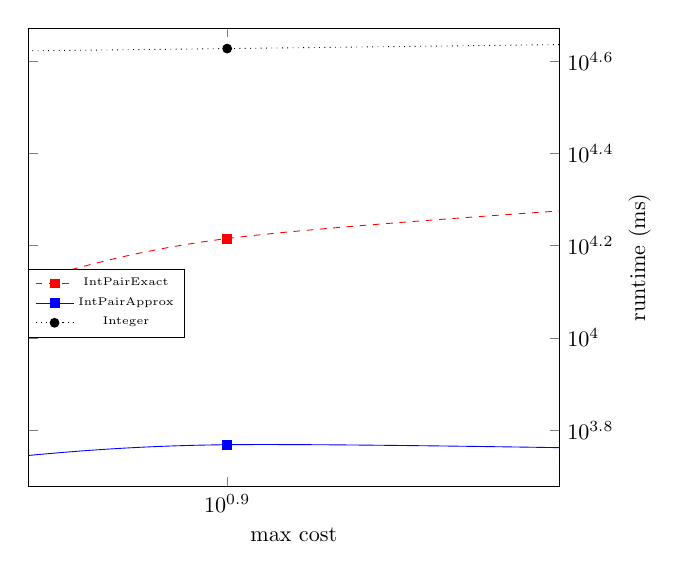
\begin{tikzpicture} [scale=0.8]
	\begin{loglogaxis}[
	yticklabel pos=right,
	  xtick=data,
	  ylabel=runtime (ms),
  	 xlabel=max cost,
	  ymin=0, ymax=47000 ] 
		\addplot[smooth,mark=square*,mark options={solid},red, dashed]
		  coordinates{ (2,4669) (4,6994) (6,9594) (8,16423) (15,22621)
		}; \label{IntPairExact Run}
		\addplot[smooth,mark=square*,mark options={solid},blue]
		  coordinates{ (2,5423) (4,5143)(6,5069) (8,5862) (15,5452)
		}; \label{IntPairApprox Run}
		\addplot[smooth,mark=*,mark options={solid},black, dotted]
		  coordinates{ (2,33288) (4,38731) (6,41307) (8,42426) (15,44868)
		}; \label{IntegerRun}
		\addlegendentry{IntPairExact}
		\addlegendentry{IntPairApprox}
		\addlegendentry{Integer}
	\end{loglogaxis}
\end{tikzpicture}
\caption{{Steps=20, Tokens=5, Steps=7. }}\label{fig:cost}
\end{figure}

%steps
\begin{figure}[H]
\centering
	\pgfplotsset{
	    scale only axis,
		legend style={at={(0,0.4)}, anchor=west, font=\tiny},
	    xmin=7, xmax=10
	}
\begin{tikzpicture} [scale=0.8] 
	\begin{axis}[
	  ylabel=nodes,
	  xtick=data,
  	  ymin=2, ymax=120000000,
  	  xlabel=steps ]
		\addplot[smooth,mark=square*, mark options={solid},red, dotted]
		  coordinates{ (7,93227)  (8,431051) (9,1992011) (10,9207489)
		}; \label{pnt_plot} \addlegendentry{IntPair}
		\addplot[smooth,mark=*,mark options={solid},black, dashed]
		  coordinates{ (7,755629)(8,3924361)(9,20128261) (10,102243101)
		}; \label{int_plot} \addlegendentry{Integer}
	\end{axis}
\end{tikzpicture}
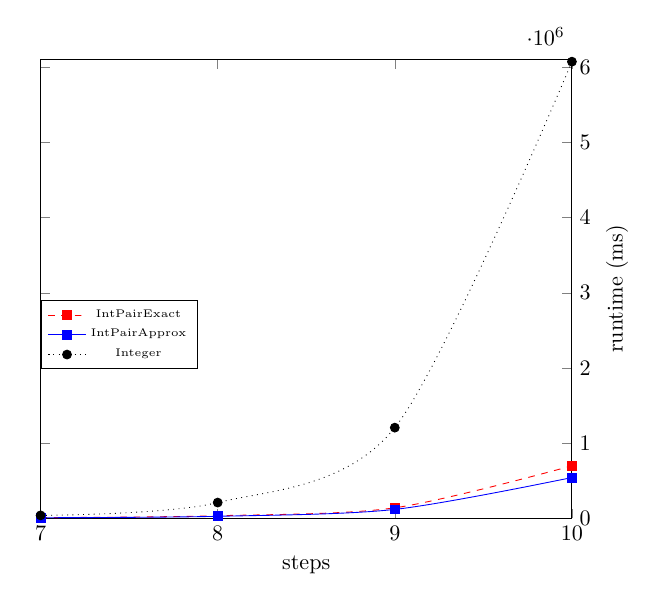
\begin{tikzpicture} [scale=0.8]
	\begin{axis}[
	yticklabel pos=right,
	  xtick=data,
	  ylabel=runtime (ms),
  	 xlabel=steps,
	  ymin=0, ymax=6100000] 
		\addplot[smooth,mark=square*,mark options={solid},red, dashed]
		  coordinates{ (7,6535) (8,32150) (9,137846) (10,696655)
		}; \label{IntPairExact Run}
		\addplot[smooth,mark=square*,mark options={solid},blue]
		  coordinates{ (7,5582)(8,24569)(9,116613) (10,540708)
		}; \label{IntPairApprox Run}
		\addplot[smooth,mark=*,mark options={solid},black, dotted]
		  coordinates{ (7,37169) (8,207591) (9,1204695)(10,6076224)
		}; \label{IntegerRun}
		\addlegendentry{IntPairExact}
		\addlegendentry{IntPairApprox}
		\addlegendentry{Integer}
	\end{axis}
\end{tikzpicture}
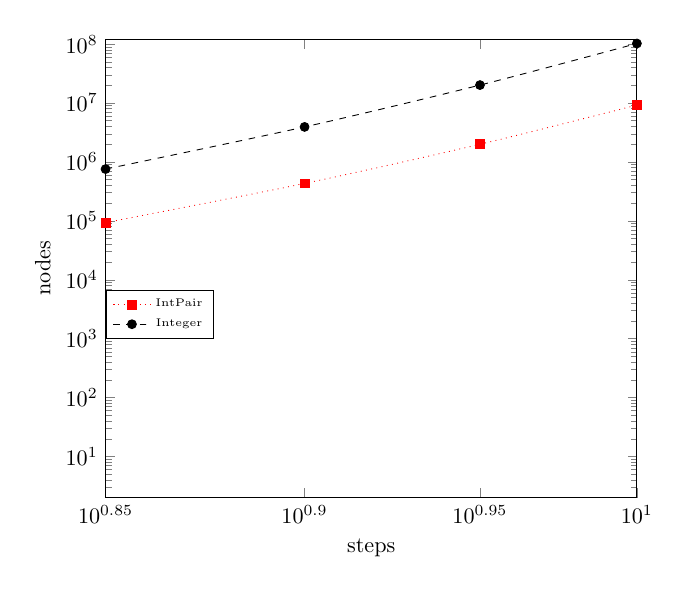
\begin{tikzpicture} [scale=0.8] 
	\begin{loglogaxis}[
	  ylabel=nodes,
	  xtick=data,
  	  ymin=2, ymax=120000000,
  	  xlabel=steps ]
		\addplot[smooth,mark=square*, mark options={solid},red, dotted]
		  coordinates{ (7,93227)  (8,431051) (9,1992011) (10,9207489)
		}; \label{pnt_plot} \addlegendentry{IntPair}
		\addplot[smooth,mark=*,mark options={solid},black, dashed]
		  coordinates{ (7,755629)(8,3924361)(9,20128261) (10,102243101)
		}; \label{int_plot} \addlegendentry{Integer}
	\end{loglogaxis}
\end{tikzpicture}
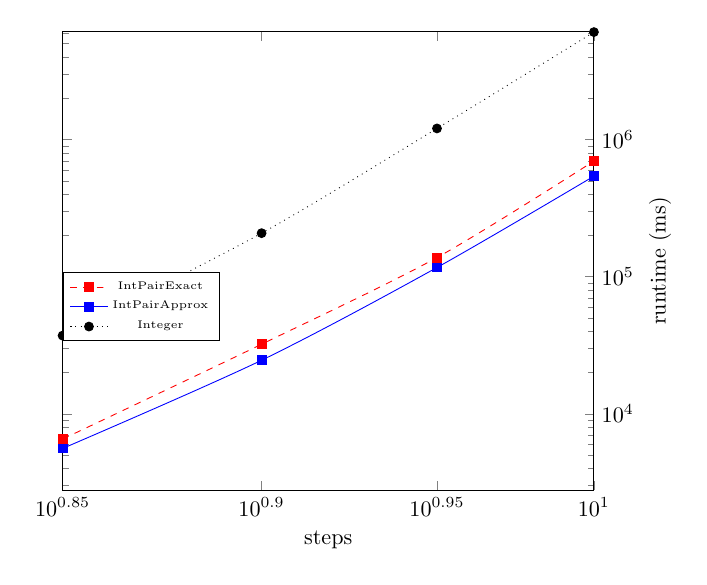
\begin{tikzpicture} [scale=0.8]
	\begin{loglogaxis}[
	yticklabel pos=right,
	  xtick=data,
	  ylabel=runtime (ms),
  	 xlabel=steps,
	  ymin=0, ymax=6100000] 
		\addplot[smooth,mark=square*,mark options={solid},red, dashed]
		  coordinates{ (7,6535) (8,32150) (9,137846) (10,696655)
		}; \label{IntPairExact Run}
		\addplot[smooth,mark=square*,mark options={solid},blue]
		  coordinates{ (7,5582)(8,24569)(9,116613) (10,540708)
		}; \label{IntPairApprox Run}
		\addplot[smooth,mark=*,mark options={solid},black, dotted]
		  coordinates{ (7,37169) (8,207591) (9,1204695)(10,6076224)
		}; \label{IntegerRun}
		\addlegendentry{IntPairExact}
		\addlegendentry{IntPairApprox}
		\addlegendentry{Integer}
	\end{loglogaxis}
\end{tikzpicture}
\caption{{States=20, Tokens=5, Maxcost=4}}\label{fig:steps}
\end{figure}

 
